\documentclass[]{standalone}
\usepackage{tikz}
\usetikzlibrary{shapes,arrows,calc,positioning}
\usepackage{amsmath} % for dfrac
\usepackage{comment}
\usepackage{calc}

% Decision
\tikzstyle{decision} = [diamond, aspect=1.8, minimum width=2cm, minimum height=1cm, text centered, text width=2cm, draw=black]

% definition of basic block
\tikzset{
    block/.style = {draw, rectangle,
        minimum height=1.2cm,
        minimum width=2cm},
    input/.style = {coordinate,node distance=1cm},
    output/.style = {coordinate,node distance=1cm},
    sum/.style = {draw, circle, node distance=1cm},
}

% definition of saturation block
\tikzset{% from https://tex.stackexchange.com/questions/161075/saturation-block
  saturation block/.style={%
    draw, 
    path picture={
      % Get the width and height of the path picture node
      \pgfpointdiff{\pgfpointanchor{path picture bounding box}{north east}}%
        {\pgfpointanchor{path picture bounding box}{south west}}
      \pgfgetlastxy\x\y
      % Scale the x and y vectors so that the range
      % -1 to 1 is slightly shorter than the size of the node
      \tikzset{x=\x*.4, y=\y*.4}
      %
      % Draw annotation
      \draw (-1,0) -- (1,0) (0,-1) -- (0,1); 
      \draw (-1,-.7) -- (-.6,-.7) -- (.6,.7) -- (1,.7);
    }
  }
}
\tikzset{% from https://tex.stackexchange.com/questions/161075/saturation-block
  deadband block/.style={%
    draw, 
    path picture={
      % Get the width and height of the path picture node
      \pgfpointdiff{\pgfpointanchor{path picture bounding box}{north east}}%
        {\pgfpointanchor{path picture bounding box}{south west}}
      \pgfgetlastxy\x\y
      % Scale the x and y vectors so that the range
      % -1 to 1 is slightly shorter than the size of the node
      \tikzset{x=\x*.4, y=\y*.4}
      %
      % Draw annotation
      \draw (-1,0) -- (1,0) (0,-1) -- (0,1);  % axis
      \draw (-1,1) -- (-.3,.3) -- (-.3,0) -- (.3,0) -- (.3,-.3) -- (1,-1);
	  %\draw (-.3,.3) -- (.3,-.3) ;
    }
  }
}

\begin{document}
	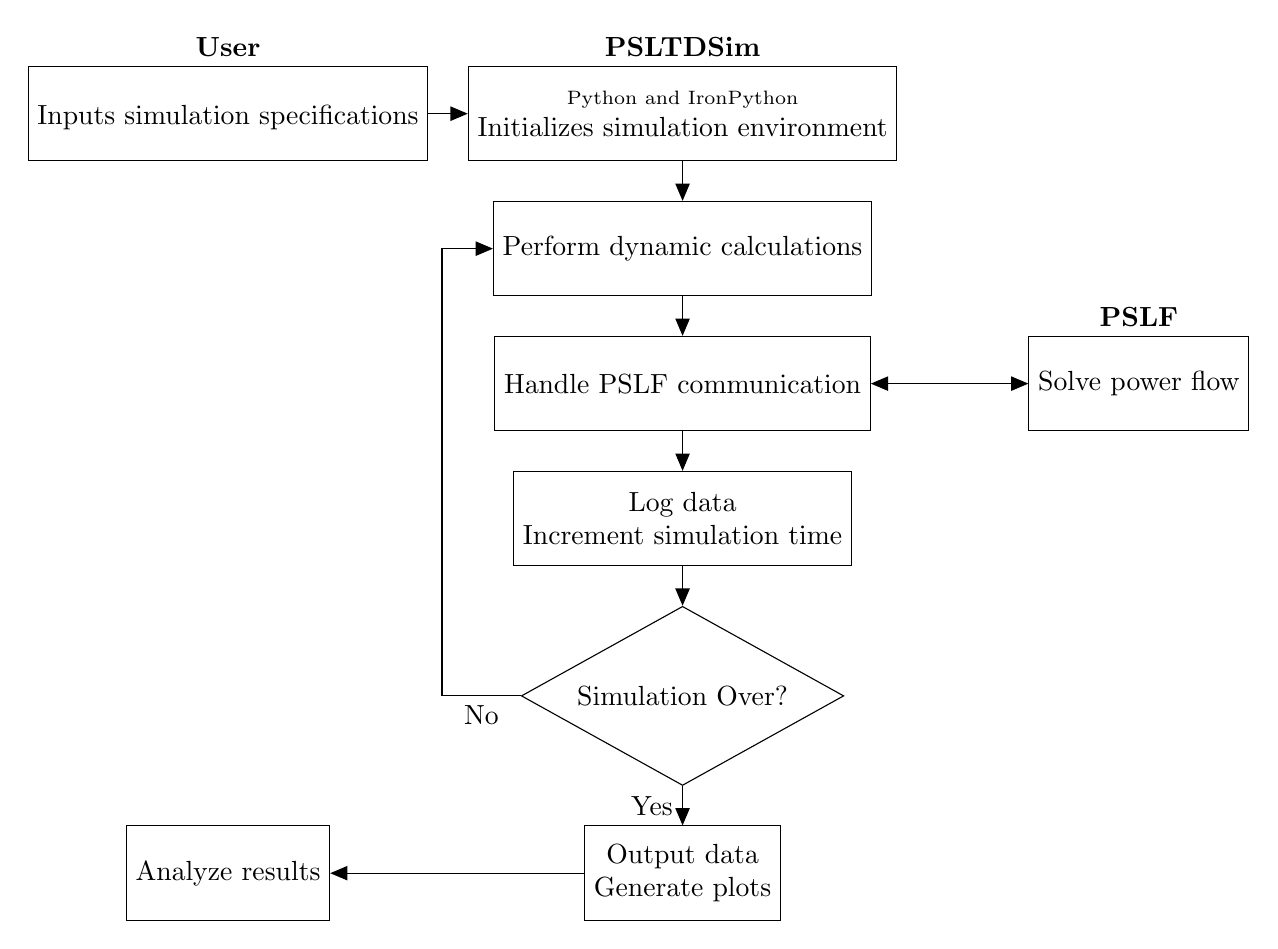
\begin{tikzpicture}[auto, node distance=.5cm,>=triangle 45]
		
		
		% user
		\node [block, label=\textbf{User}] (user) {\shortstack{\\ Inputs simulation specifications}};
		
		
		% python init
		\node [block, right=of user,label=\textbf{PSLTDSim} ] (python) {\shortstack{{\scriptsize Python and IronPython}\\ Initializes simulation environment}};
		% python loop
		\node [block, below=of python,] (pythonloop1) {\shortstack{Perform dynamic calculations}};
		
		\node [block, below=of pythonloop1,] (pythonloop2) {\shortstack{Handle PSLF communication}};
		
		\node [block, below=of pythonloop2,] (pythonloop3) {\shortstack{Log data\\ Increment simulation time}};
		
		% sim over decision
		\node (simOver) [decision, below =of pythonloop3,text width=3cm] {Simulation Over?};
		
		% python output
		\node [block, below=of simOver,] (pythonoutput) {\shortstack{Output data \\ Generate plots}};
		
		% pslf
		\node [block, right=2cm of pythonloop2, label=\textbf{PSLF} ] (pslf) {\shortstack{Solve power flow}};
		
		% analyze
	%	\coordinate (2ndUser) at ($ , $)
		\node [block] (userout) at (pythonoutput -| user) {\shortstack{Analyze results}};

		\draw [->] (user) -- (python);
		\draw [->] (python) -- (pythonloop1);
		\draw [->] (pythonloop1) -- (pythonloop2);
		\draw [->] (pythonloop2) -- (pythonloop3);
		\draw [<->] (pythonloop2) -- (pslf);
		\draw [->] (pythonloop3) -- (simOver);
		\draw [->] (pythonoutput) -- (userout);
		
		% pf convergence bad
		\draw [->] (simOver) --  node[anchor=east] {Yes} (pythonoutput);
		\draw (simOver.west) -- node[anchor=north] {No} ($(simOver.west) + (-1,0)$);
		\draw [->] ($(simOver.west) + (-1,0)$) |- (pythonloop1.west);

	\end{tikzpicture} 
\end{document}